\documentclass[conference]{IEEEtran}
\IEEEoverridecommandlockouts
% The preceding line is only needed to identify funding in the first footnote. If that is unneeded, please comment it out.
\usepackage{cite}
\usepackage{amsmath,amssymb,amsfonts}
\usepackage{algorithmic}
\usepackage{graphicx}
\usepackage{textcomp}
\usepackage{xcolor}
\def\BibTeX{{\rm B\kern-.05em{\sc i\kern-.025em b}\kern-.08em
    T\kern-.1667em\lower.7ex\hbox{E}\kern-.125emX}}
\begin{document}

\title{Microgrid Project\\}

\author{\IEEEauthorblockN{Jesse Both}
\IEEEauthorblockA{\textit{Department of Computer Science and Engineering} \\
\textit{University at Buffalo}\\
Buffalo, New York \\
jessebot@buffalo.edu}}

\maketitle

\begin{abstract}
    Microgrid optimization is a complex topic that computational intelligence techniques can be used. This paper will explore a microgrid optimization using a genetic algorithm.  There are two types of reproduction methods: mutation and crossover as well as 2 types of survival methods: elitism and random selection that will be explored to determine which combination of methods produces the best results.
\end{abstract}
\begin{IEEEkeywords}
Microgrid, Genetic Algorithm, gene, chromosome
\end{IEEEkeywords}

\section{Introduction}
    Microgrids are self sufficient power distribution systems.  In order to be self sufficient, the system needs an intelligent controller to determine where the power should come from.  In this paper, a microgrid controller implementation will be explored using a genetic algorithm.  There will be two types of survival methods and two types of reproduction methods that will be analyzed and compared to see what solution combination of methods can give the best results. The reproduction methods that will be used are mutation and crossover.  The survival methods that will be utilized are elitism and random selection.

\section{Design}
    \subsection{Microgrid Block Diagram}
    \begin{figure}[h!]
    \begin{center}
        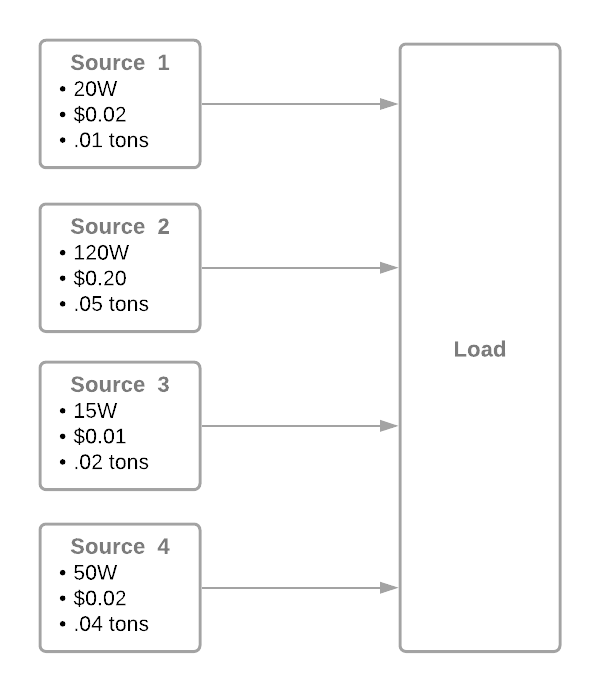
\includegraphics[height=6cm]{graphics/block_diagram.png}
    \end{center}
    \caption{Block Diagram}
    \label{fig:block}
    \end{figure}

    \subsection{Load Time Series}
    This time series was designed by deciding with the idea that the power is being sent to a residential area.  The usage would be low in the middle
    of the night and high when residents are home from work.  It would gradually
    increase/decrease throughout the other parts of the day.  The assumption
    is that a week days are being explored.

    To find the values, a range was given for each hour through out the day.
    A value for each hour within these ranges is randomly selected.  A set
    number of days can be produced.  In order to smooth out the curve an additional parameter was utilized to combine a set of days into a group and take the mean.  The purpose of this is to smooth out the curve into something that would look more realistic.

    \subsection{Source Chromosome Format}
    The chromosome format for each source is
    \[[cost, emission]\]

    The defined boundaries are:
    \begin{itemize}
        \item \(15W \leq power \leq 100W\)
        \item \(\$.15 \leq cost \leq \$6.55\)
        \item \(.15 tons \leq emission \leq 3.75 tons\)
    \end{itemize}

    \subsection{Fitness Optimization}
    Economic optimization means that lower cost is better.  If the requirements can be met with lower cost this would be a beneficial economic adjustment.

    Economic boundary for fitness function are [0, 1], 0 being the best.
    \newline 

    Environmental optimization would imply that less emissions produced would be better for the environment.

    Environmental boundary for fitness function are [0, 1], 0 being the best.
    \newline 

    The equation used to find the fitness of these optimizations is:
    \[W*\frac{cost-min}{max-min}\]

    Another optimization that is required is the amount of power is delivered.  If there is not enough power being delivered then outages will occur.

    \subsection{Defined Constants}
    The population size that will be used is 100 chromosomes with a mutation rate of .1.  The stopping condition for the fitness function is .08.  the cross over point that will be used is 2.

    \section{Genetic Algorithm}
    \subsection{Algorithm Flow}
        \begin{figure}[h!]
            \begin{center}
                \includegraphics[height=10cm]{graphics/GA.png}
            \end{center}
            \caption{Flow Chart}
            \label{fig:gaflow}
        \end{figure}

    \subsection{Reproduction Methods}
    \subsubsection{Mutation}
    For mutation to occur, first random chromosomes in the population are selected to be mutated.  If the produced chromosome is feasible it is added into the population.  The genes that are selected are chosen at random.
    \subsubsection{Crossover}
    In crossover, two parents are randomly selected to be used to reproduce.  Two children are produced corresponding to the crossover point. The crossover point is the point at which the parent chromosomes are split and which genes the children inherit.
    \subsection{Survival Methods}
    \subsubsection{Elitism}
    Elitism reduces the population to the correct population size by killing off less ideal chromosomes.  This is done by looking at the fitness of each function at removing the chromosomes with the worst fitness.
    \subsubsection{Random Selection}
    Random selection reduces the population by randomly selecting chromosomes to kill off.  This is done by creating a random permutation of indices to determine which chromosomes should be remove.

    \section{Analysis}
    \subsection{Excess Power}
    It can be seen that the random mutations causes an increased amount of excess power that is produced due to its random nature.  Random selection also hinders the excess power even further when combined with random mutation. When mutation is paired with elitism, the results are slightly more efficient.  When crossover is combined with random selection, the results are similar to mutation due to its lack of diversity.  When crossover is combined with elitism, the best result are made due to only reproducing with the most elite chromosome for each generation.

    \subsection{Cost}
    The cost for each method is quite similar and behaves as you might expect.  The cost throughout the day typically follows the trend of the power output.
    the typical range for cost is \(\$50 \leq cost \leq \$65\)

    \subsection{Environmental Impact}
    The emissions also follows a similar trend to the power across all methods.  interestingly, the curve is typically a little wider than that of the power curve. Perhaps this is due to the defined weights. The range for emissions is typically \(40 \leq emissions \leq 48 \) tons

    \subsection{Calculation Time}
    The time it took to generate across all methods was quite predictable.  
    The main driving factor that hindered the calculation time was the survival method.  Random selection typically took longer than that of elitism.  Interestingly, the difference between mutation and crossover time was not that different as long as the crossover set received a good starting point. There are some cases where crossover is unsolvable due to lack of diversity.

    \section{Recommendation}

    \subsection{Improvements}
    The initial chromosome generation could be optimized to use more realistic values and diverse.  Crossover benefits from larger data sets with more diversity as a starting point.  If the original chromosomes were intentionally more diverse there could be better results.  In the case that the good enough value is too low or the data set is not diverse enough the algorithm will run out of solutions to make it to the stopping condition.


    \subsection{Concerns to Be Addressed}
    One concern that is not addressed in this system is that there is no value for the maximum heat that the sources can produce before failure.  With this additional constraint there may be times were it would be more logical to increase cost and/or emissions in order to cool a source that has done a lot of work.  With the way the system is set up now, a source could go all day without any down time while another source doesn't do much.  The lack of this information could lead to catastrophic failure.

    Another concern is that there is no set limit how much extra power can be produced.  With no location for storage, the system could over load the load and could potentially cause fires or explosions depending on how much excess power is sent to the load.

    \section{Conclusion}
    Genetic algorithms can be a great way to automate systems, but typically their output is not the best possible solution that can occur.  This is good for situations that require automation that their are not strict constraints on performance.  Genetic algorithms perform better when there are more genes to deal with where a human may not be able to calculate the best possible result by hand.  

\end{document}
